\documentclass[aspectratio=169,xcolor=pdftex,dvipsnames,table]{beamer}\usepackage[]{graphicx}\usepackage[]{xcolor}
% maxwidth is the original width if it is less than linewidth
% otherwise use linewidth (to make sure the graphics do not exceed the margin)
\makeatletter
\def\maxwidth{ %
  \ifdim\Gin@nat@width>\linewidth
    \linewidth
  \else
    \Gin@nat@width
  \fi
}
\makeatother

\definecolor{fgcolor}{rgb}{0.345, 0.345, 0.345}
\newcommand{\hlnum}[1]{\textcolor[rgb]{0.686,0.059,0.569}{#1}}%
\newcommand{\hlsng}[1]{\textcolor[rgb]{0.192,0.494,0.8}{#1}}%
\newcommand{\hlcom}[1]{\textcolor[rgb]{0.678,0.584,0.686}{\textit{#1}}}%
\newcommand{\hlopt}[1]{\textcolor[rgb]{0,0,0}{#1}}%
\newcommand{\hldef}[1]{\textcolor[rgb]{0.345,0.345,0.345}{#1}}%
\newcommand{\hlkwa}[1]{\textcolor[rgb]{0.161,0.373,0.58}{\textbf{#1}}}%
\newcommand{\hlkwb}[1]{\textcolor[rgb]{0.69,0.353,0.396}{#1}}%
\newcommand{\hlkwc}[1]{\textcolor[rgb]{0.333,0.667,0.333}{#1}}%
\newcommand{\hlkwd}[1]{\textcolor[rgb]{0.737,0.353,0.396}{\textbf{#1}}}%
\let\hlipl\hlkwb

\usepackage{framed}
\makeatletter
\newenvironment{kframe}{%
 \def\at@end@of@kframe{}%
 \ifinner\ifhmode%
  \def\at@end@of@kframe{\end{minipage}}%
  \begin{minipage}{\columnwidth}%
 \fi\fi%
 \def\FrameCommand##1{\hskip\@totalleftmargin \hskip-\fboxsep
 \colorbox{shadecolor}{##1}\hskip-\fboxsep
     % There is no \\@totalrightmargin, so:
     \hskip-\linewidth \hskip-\@totalleftmargin \hskip\columnwidth}%
 \MakeFramed {\advance\hsize-\width
   \@totalleftmargin\z@ \linewidth\hsize
   \@setminipage}}%
 {\par\unskip\endMakeFramed%
 \at@end@of@kframe}
\makeatother

\definecolor{shadecolor}{rgb}{.97, .97, .97}
\definecolor{messagecolor}{rgb}{0, 0, 0}
\definecolor{warningcolor}{rgb}{1, 0, 1}
\definecolor{errorcolor}{rgb}{1, 0, 0}
\newenvironment{knitrout}{}{} % an empty environment to be redefined in TeX

\usepackage{alltt}
% \documentclass[notes,aspectratio=169,xcolor=pdftex,dvipsnames,table]{beamer}

%\setbeameroption{show notes}

\usepackage{bm,graphicx,amsmath,tikz} %fancybox,
\usepackage{color}%,textpos}
\usepackage[round]{natbib}
\usepackage[normalem]{ulem}
\usepackage{hyperref}
\usepackage{lastpage}
\usepackage{array}
\usepackage{color}
\usepackage{framed}

% Define Western colours
\definecolor{western}{rgb}{.306,.152,.524}
\definecolor{westerngray}{rgb}{.512,.508,.524}

%% Define BEAMER colours
\setbeamercolor{frametitle}{bg=western,fg=white}
\setbeamercolor{framesubtitle}{bg=western,fg=black}
\setbeamercolor{title}{fg=white,bg=western}
\setbeamercolor{author}{fg=white,bg=western}
\setbeamercolor{institute}{fg=white,bg=western}
\setbeamercolor{date}{fg=white,bg=western}

%% Set BEAMER fonts
\setbeamerfont{title}{shape=\bf}
\setbeamerfont{frametitle}{shape=\sc,size=\Large}
\setbeamerfont{framesubtitle}{shape=\sc,size=\Large}
\setbeamerfont{footline}{shape=\sc}

%% Define BEAMER toc
\setbeamercolor{section in toc}{fg=western}
\setbeamercolor{subsection in toc}{fg=westerngray}
\setbeamertemplate{sections/subsections in toc}[ball]

%% Define BEAMER background
\setbeamercolor{background canvas}{bg=white}

%% Define BEAMER footer
\setbeamertemplate{navigation symbols}{}
\setbeamercolor{footline}{fg=white,bg=western}
\setbeamertemplate{footline}{%
  \begin{beamercolorbox}[wd=\paperwidth]{footline}
    \vskip5pt

    \hspace{.1in}
    \raisebox{.05in}{
      \scriptsize{\bf \insertshorttitle }
    }
    \hfill
    \raisebox{.05in}{
      \scriptsize{\bf \insertframenumber/\inserttotalframenumber}
    }
    \hspace{5pt}

    \vskip5pt
  \end{beamercolorbox}
}

%% Define BLOCK environment
\setbeamercolor{block title}{fg=western}
\setbeamerfont{block title}{series=\bfseries}

%% Define ENUMERATE and ITEMIZE environements
\setbeamertemplate{itemize item}[ball]
\setbeamertemplate{enumerate item}[ball]
\setbeamercolor{item projected}{bg=western}

%% Define BEAMER toc
\setbeamercolor{sections/subsections in toc}{fg=blue!75}
\setbeamertemplate{sections/subsections in toc}[ball]

%% Define SECTION openings
\AtBeginSection[]{
}

\title[SS2857 -- Lecture 5]{SS2857 Probability and Statistics 1\\
  Fall 2021\\
  \vspace{.2in}
  Lecture 5}

\date{}



\IfFileExists{upquote.sty}{\usepackage{upquote}}{}
\begin{document}

{
\setbeamertemplate{footline}{}
\setbeamercolor{background canvas}{bg=western}

\begin{frame}
  \maketitle
\end{frame}
}


\begin{frame}
  \begin{center}
    \Large{\textbf{2.5 Independence}}

    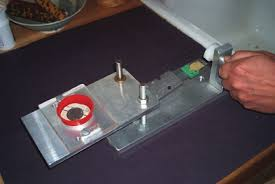
\includegraphics[height = .6\textheight]{Figures/coin_tossing_machine.jpg}
    

  \end{center}
  
    \begin{small}
    Persi Diaconis, Susan Holmes, and Richard Montgomery (2007) \textit{Dynamical Bias in the Coin Toss}. SIAM Review 2007 49:2, 211-235
    \end{small}
\end{frame}

\begin{frame}{Independence}
  Two events, $A$ and $B$, are independent if the conditional probability of $A$ given $B$ is equal to the probability of $A$, or vice versa:
  \[
    P(A|B)=P(A) \mbox{ or } P(B|A)=P(B).
  \]
  Two events that are not independent are dependent.
\end{frame}

\begin{frame}{Example 5.1}
  Suppose that $A$ and $B$ are disjoint events with positive probability ($P(A)>0$ and $P(B)>0$).

  \begin{center}
    Can they be independent?
  \end{center}
\end{frame}

\begin{frame}{Example 5.2}
  
    Which pairs of events do you think are independent? Explain.

    \begin{enumerate}[a)]
    \item A: It rains in London, Ontario, on October 1.\\
      B: It rains in London, Ontario, on October 2.
    \item A: It rains in London, Ontario, on October 1, 2022.\\
      B: It rains in London, England, on October 1, 2023.
    \item A: Erin scores $>80\%$ on an exam.\\
      B: Jonah scores $>80\%$ on the same exam.
    \item A: The Yankees win the baseball World Series.\\
      B: The Royals win the baseball World series.
    \end{enumerate}

\end{frame}

\begin{frame}{Independence II}
  Two events $A$ and $B$ are independent if and only if
  \[
    P(A \cap B) = P(A) P(B).
  \]
\end{frame}

\begin{frame}{Example 5.3}
  Let $A$ and $B$ be two events such that
  \begin{enumerate}[i)]
  \item $P(A \cap B')=.15$
  \item $P(A' \cap B')=.35$
  \item $P(A' \cap B)=.35$
  \end{enumerate}

  \medskip

  Are $A$ and $B$ independent?
\end{frame}

\begin{frame}{Example 5.4}

Show that if $A'$ and $B'$ are independent then $A$ and $B$ are also independent. 

\end{frame}

\begin{frame}{Mutually Independent}
  Several events are mutually independent if the probability of the intersection of any collection of the events is the product of the probabilities of the individual events.

  \bigskip

  Mathematically, $A_1,\ldots,A_n$ are mutually independent if
  \[
    P(\cap_{i \in \mathcal I} A_i)=\prod_{i \in \mathcal I} P(A_i)
  \]
  for any subset $\mathcal I \subset \{1,\ldots,n\}$. 
\end{frame}

\begin{frame}
  \begin{center}
    \Large{\textbf{Questions?}}
  \end{center}
\end{frame}

\begin{frame}{Exercise 5.1}
  Suppose that you toss a fair coin $n$ times and count the number of heads.

  \medskip

  \begin{enumerate}[a)]
  \item Let $H_i$ be the event that the coin lands heads side up on the $i$-th toss. What does it mean for $H_1$ and $H_2$ to be independent?
  \item Does independence necessarily mean that the coin is fair?
  \item What does it mean for the events $H_1,\ldots,H_n$ to be mutually independent?
  \item What is the probability that the coin lands heads-side up on every one of $n=10$ tosses?
  \item What is the probability that the tosses alternate between landing heads-side up first then tails-side up etc if $n=10$?
  \item What is the probability that the coin lands heads-side up 5 times if $n=10$?
  \end{enumerate}
\end{frame}

\end{document}
